\documentclass[a4paper, twocolumn]{article}
\usepackage[pdftex, hidelinks,
            pdftitle={Machine Learning Report},
            pdfauthor={Erik Sven Vasconcelos Jansson},
            pdfsubject={Machine Learning Report},
            pdfkeywords={report}]{hyperref}

\usepackage{bm}
\usepackage[T1]{fontenc}
\usepackage[utf8]{inputenc}
\usepackage{algorithmic}
\usepackage{algorithm}
\usepackage{amsfonts}
\usepackage{booktabs}
\usepackage{amssymb}
\usepackage{courier}
\usepackage{booktabs}
\usepackage{graphicx}
\usepackage{listings}
\usepackage{mathtools}
\usepackage[capitalize, noabbrev]{cleveref}
\lstset{basicstyle=\footnotesize\ttfamily,
        breakatwhitespace = false,
        breaklines = true,
        keepspaces = true,
        language = R,
        showspaces = false,
        showstringspaces = false,
        belowcaptionskip = \bigskipamount,
        framerule = 0.80pt,
        frame = tb,
        numbers = left,
        belowskip = \bigskipamount,
        escapeinside={<@}{@>}}

\title{Introduction to Machine Learning \\
       Individual Laboration Report --6--}
\author{{Erik Sven Vasconcelos Jansson} \\
        {\href{mailto:erija578@student.liu.se}
        {\texttt{erija578@student.liu.se}}} \\
        {Linköping University, \, Sweden}}

\begin{document}

    \pagenumbering{arabic}
    \maketitle % Titles...

    \begin{equation} \label{eq:sigmoid}
        \sigma(u) = \frac{1}{1 + e^{-u}}
    \end{equation}

    \begin{equation} \label{eq:batch_gradient}
        \bm{w}_{(i)} = \bm{w}_{(i-1)} - \eta_k \nabla E(\bm{w}_{(i-1)})
    \end{equation}

    \begin{equation} \label{eq:perceptron}
        y_j(\bm{x}) = \sigma(w_0 + \sum_{h=1}^{H} \sigma(w_{0h} + \bm{w}_h^\intercal\bm{x}))
    \end{equation}

    \begin{figure}[h!]
        \centering
        \caption{Neural Network}
        \label{fig:network}
        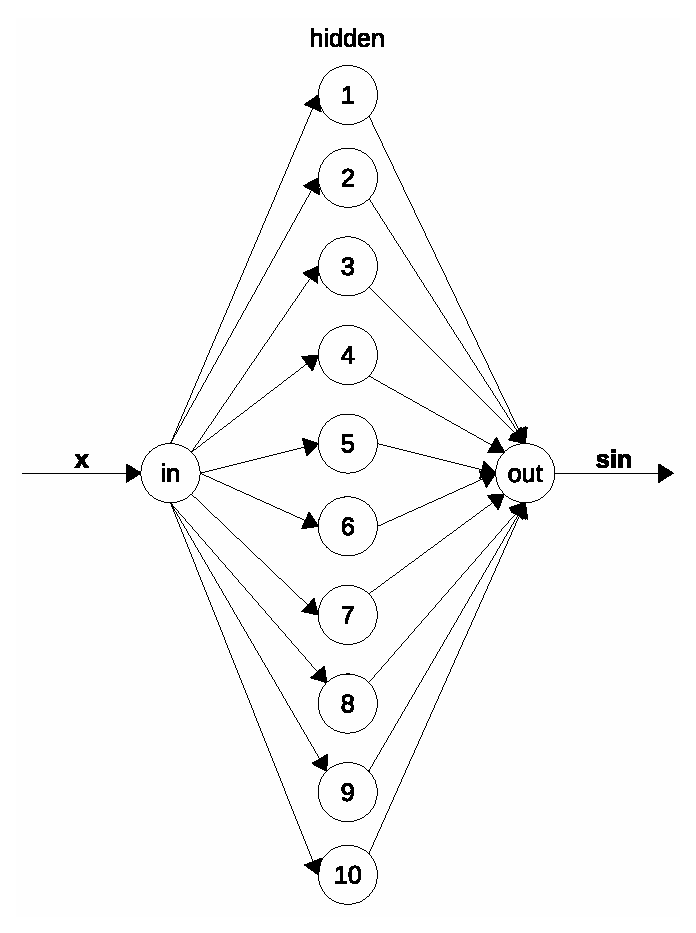
\includegraphics[width=0.5\textwidth]{share/network.eps}
    \end{figure}

    \begin{figure}[h!]
        \centering
        \caption{Neural Network Predictions}
        \label{fig:predictions}
        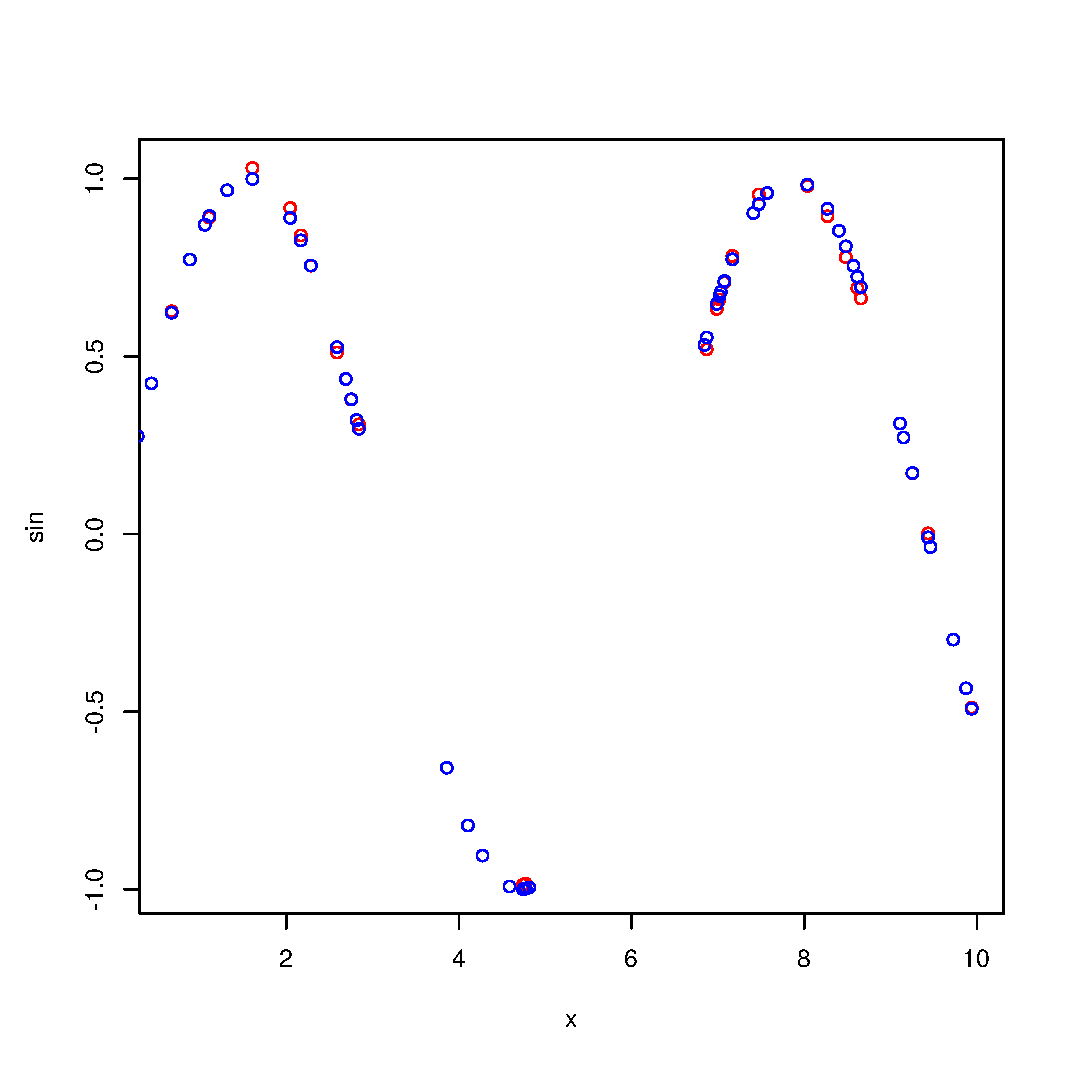
\includegraphics[width=0.5\textwidth]{share/predictions.eps}
    \end{figure}

    \begin{table}[h!]
        \begin{center}
            \begin{tabular}{cc}
                \toprule
                \textbf{Threshold} & \textbf{S.S.E.} \\
                \midrule
                0.001 & 0.01367691527 \\
                0.002 & 0.01262419958 \\
                0.003 & 0.00988418900 \\
                0.004 & 0.00850089424 \\
                0.005 & 0.00955545744 \\
                0.006 & 0.00974372099 \\
                0.007 & 0.01583926857 \\
                0.008 & 0.01649252416 \\
                0.009 & 0.02112490377 \\
                0.010 & 0.02735909554 \\
                \bottomrule
            \end{tabular}
        \end{center}
        \caption{Neural Network Values}
        \label{tab:forecast}
    \end{table}

    \nocite{*}
    \bibliographystyle{alpha}
    \bibliography{report}

    \onecolumn \appendix
    \section*{Appendix}

    \lstinputlisting[caption={Feed-Forward Backpropagating Neural Network Sine Estimator Script}, label={lst:neuralnet}]{share/neuralnet.r}

\end{document}
